\documentclass{article}
\usepackage{fullpage,booktabs,graphicx,hyperref,float,array}
% generated by grnbench report from result files - do not edit
\newcommand{\gbCiHighAuprcRatioAutoPearsonMotifVsMotifPrior}{+0.234}
\newcommand{\gbCiHighAuprcRatioAutoPearsonMotifVsPearsonSigned}{+0.227}
\newcommand{\gbCiHighAuprcRatioBaselinePearsonMotifVsMotifPrior}{+0.228}
\newcommand{\gbCiHighAuprcRatioBaselinePearsonMotifVsPearsonSigned}{+0.225}
\newcommand{\gbCiHighEprAutoPearsonMotifVsMotifPrior}{+1.184}
\newcommand{\gbCiHighEprAutoPearsonMotifVsPearsonSigned}{+0.286}
\newcommand{\gbCiHighEprBaselinePearsonMotifVsMotifPrior}{+1.154}
\newcommand{\gbCiHighEprBaselinePearsonMotifVsPearsonSigned}{+0.318}
\newcommand{\gbCiLowAuprcRatioAutoPearsonMotifVsMotifPrior}{+0.077}
\newcommand{\gbCiLowAuprcRatioAutoPearsonMotifVsPearsonSigned}{+0.138}
\newcommand{\gbCiLowAuprcRatioBaselinePearsonMotifVsMotifPrior}{+0.076}
\newcommand{\gbCiLowAuprcRatioBaselinePearsonMotifVsPearsonSigned}{+0.143}
\newcommand{\gbCiLowEprAutoPearsonMotifVsMotifPrior}{+0.495}
\newcommand{\gbCiLowEprAutoPearsonMotifVsPearsonSigned}{-0.046}
\newcommand{\gbCiLowEprBaselinePearsonMotifVsMotifPrior}{+0.491}
\newcommand{\gbCiLowEprBaselinePearsonMotifVsPearsonSigned}{-0.014}
\newcommand{\gbDiffAuprcRatioAutoPearsonMotifVsMotifPrior}{+0.155}
\newcommand{\gbDiffAuprcRatioAutoPearsonMotifVsPearsonSigned}{+0.182}
\newcommand{\gbDiffAuprcRatioBaselinePearsonMotifVsMotifPrior}{+0.152}
\newcommand{\gbDiffAuprcRatioBaselinePearsonMotifVsPearsonSigned}{+0.184}
\newcommand{\gbDiffEprAutoPearsonMotifVsMotifPrior}{+0.839}
\newcommand{\gbDiffEprAutoPearsonMotifVsPearsonSigned}{+0.120}
\newcommand{\gbDiffEprBaselinePearsonMotifVsMotifPrior}{+0.823}
\newcommand{\gbDiffEprBaselinePearsonMotifVsPearsonSigned}{+0.152}
\newcommand{\gbFamilyAuprcRatioAuto}{4}
\newcommand{\gbFamilyAuprcRatioBaseline}{4}
\newcommand{\gbFamilyEprAuto}{4}
\newcommand{\gbFamilyEprBaseline}{4}
\newcommand{\gbMeanAuprcRatioAutoMotifPrior}{1.373}
\newcommand{\gbMeanAuprcRatioAutoPearsonMotif}{1.529}
\newcommand{\gbMeanAuprcRatioAutoPearsonSigned}{1.346}
\newcommand{\gbNAuprcRatioAutoPearsonMotifVsMotifPrior}{20}
\newcommand{\gbNAuprcRatioAutoPearsonMotifVsPearsonSigned}{20}
\newcommand{\gbNAuprcRatioBaselinePearsonMotifVsMotifPrior}{20}
\newcommand{\gbNAuprcRatioBaselinePearsonMotifVsPearsonSigned}{20}
\newcommand{\gbNAutoMotifPrior}{20}
\newcommand{\gbNAutoPearsonMotif}{20}
\newcommand{\gbNAutoPearsonSigned}{20}
\newcommand{\gbNDatasets}{20}
\newcommand{\gbNEprAutoPearsonMotifVsMotifPrior}{20}
\newcommand{\gbNEprAutoPearsonMotifVsPearsonSigned}{20}
\newcommand{\gbNEprBaselinePearsonMotifVsMotifPrior}{20}
\newcommand{\gbNEprBaselinePearsonMotifVsPearsonSigned}{20}
\newcommand{\gbPHolmAuprcRatioAutoPearsonMotifVsMotifPrior}{0.00083}
\newcommand{\gbPHolmAuprcRatioAutoPearsonMotifVsPearsonSigned}{1.4e-07}
\newcommand{\gbPHolmAuprcRatioBaselinePearsonMotifVsMotifPrior}{0.00073}
\newcommand{\gbPHolmAuprcRatioBaselinePearsonMotifVsPearsonSigned}{2.9e-08}
\newcommand{\gbPHolmEprAutoPearsonMotifVsMotifPrior}{0.00013}
\newcommand{\gbPHolmEprAutoPearsonMotifVsPearsonSigned}{0.219}
\newcommand{\gbPHolmEprBaselinePearsonMotifVsMotifPrior}{0.0001}
\newcommand{\gbPHolmEprBaselinePearsonMotifVsPearsonSigned}{0.105}
\newcommand{\gbPHolmRevAuprcRatioAutoPearsonMotifVsMotifPrior}{1.000}
\newcommand{\gbPHolmRevAuprcRatioAutoPearsonMotifVsPearsonSigned}{1.000}
\newcommand{\gbPHolmRevAuprcRatioBaselinePearsonMotifVsMotifPrior}{1.000}
\newcommand{\gbPHolmRevAuprcRatioBaselinePearsonMotifVsPearsonSigned}{1.000}
\newcommand{\gbPHolmRevEprAutoPearsonMotifVsMotifPrior}{1.000}
\newcommand{\gbPHolmRevEprAutoPearsonMotifVsPearsonSigned}{1.000}
\newcommand{\gbPHolmRevEprBaselinePearsonMotifVsMotifPrior}{1.000}
\newcommand{\gbPHolmRevEprBaselinePearsonMotifVsPearsonSigned}{1.000}

\title{EXP-20260925-LM-2: Confirmatory - does the motif prior lift GRN recovery on fresh real datasets?}
\author{grnbench report generated from EXP-20260925-LM-2}
\date{}
\begin{document}
\maketitle
\section*{Status}
Experiment EXP-20260925-LM-2, type: confirmatory. Record status: registered. Reproduced by: nobody yet.
\section{Configuration summary}
\begin{table}[H]\centering\small
\caption{Configuration of the run, from the experiment record and the run folder.}
\begin{tabular}{p{0.3\linewidth}p{0.62\linewidth}}\toprule
experiment & EXP-20260925-LM-2 \\
type & **confirmatory** (pre-registration = the commit that adds this file, pushed before any dataset of this list was downloaded or scored) \\
owner & LM   issue: board issue opened at launch   registered: 2026-09-25 \\
datasets (rows) & 20 \\
models & motif\_prior, pearson\_motif, pearson\_signed \\
arms & auto, baseline \\
code & branch lm/confirmatory-motif-prior, commit recorded in the results folder (CODE\_COMMIT), which includes the scrublet fix (PR \#3: scikit-image present, doublet fallback recorded per arm) and real\_bench --keep-artifacts for the explainability figures. \\
code commit (run folder) & 67ca8809661baf5c4982a407805cccae2ebcf002 \\
environment & fresh venv from requirements/lock-py311.txt (Python 3.11.9, Windows), no torch. \\
machine & local laptop (Windows, 3 workers) \\
seeds & reference split seed 0 (screen.split\_reference), cell subsample seed 0 (at most 3,000 cells per context, MAX\_SCORE\_CELLS), scrublet seed 0; regulators = the 150 TFs with most reference targets in the data (MAX\_TFS). \\
run folder & benchmarks/results/EXP-20260925-LM-2 \\
generated & 2026-09-25 19:50 \\
\bottomrule\end{tabular}\end{table}

\section{Methods}
\begin{description}
\item[type] **confirmatory** (pre-registration = the commit that adds this file, pushed before any dataset of this list was downloaded or scored)
\item[primary endpoint] AUPRC ratio (AUPRC / prevalence; 1 = random) on the CollecTRI evaluation half, **auto** pipeline arm (the engine's screened choice), mean over contexts within a dataset. pearson\_motif vs motif\_prior (does expression add to the prior alone).
\item[unit of analysis] dataset. Planned n = 20 (list below); analysed n = datasets with a score for both members of a pair (printed per pair).
\item[datasets] experiments/EXP-20260925-LM-2.datasets.tsv (20 CELLxGENE Discover datasets, human 16 / mouse 4, 8 protocols), chosen by benchmarks/fetch\_cellxgene.py --max 20 --max-mb 60 --organisms "Homo sapiens,Mus musculus" --exclude-ids experiments/EXP-20260925-LM-2.excluded\_ids.txt --exclude-assay targeted on the public listing of 2026-09-25. Excluded before selection: the 31 dataset ids used by any earlier experiment (EXP-20260925-LM-2.excluded\_ids.txt) and targeted panels (not transcriptomes).
\item[exclusion rules (fixed now)] (a) a dataset whose download fails or whose sha256 cannot be recorded is replaced by nobody and reported as missing; (b) datasets with fewer than 50 reference edges among their genes are not scored (MIN\_REFERENCE\_EDGES, as in the code); (c) a dataset where a model errors is dropped from the pairs involving that model only, and reported; (d) no other exclusion, no outlier removal.
\item[comparison family] real\_bench.DECLARED\_PAIRS restricted to the models run = \{(pearson\_motif, pearson\_signed), (pearson\_motif, motif\_prior)\}, both directions = 4 directed hypotheses per metric and arm.
\item[test] paired t over datasets, two-sided per direction, via compare\_units for each pair (95\% interval of the mean paired difference), Holm over the 4 directed hypotheses of the AUPRC / auto family, alpha 0.05. **H1 is supported** if p\_Holm(pearson\_motif > pearson\_signed) < 0.05 in that family; **refuted** if p\_Holm(pearson\_signed > pearson\_motif) < 0.05; otherwise inconclusive.
\item[seeds] reference split seed 0 (screen.split\_reference), cell subsample seed 0 (at most 3,000 cells per context, MAX\_SCORE\_CELLS), scrublet seed 0; regulators = the 150 TFs with most reference targets in the data (MAX\_TFS).
\item[models] pearson\_signed, pearson\_motif, motif\_prior. RegDiffusion is **not** run: about 13 min per dataset per arm on this CPU (about 9 h for 20 datasets x 2 arms), it goes to an HPC experiment.
\item[code] branch lm/confirmatory-motif-prior, commit recorded in the results folder (CODE\_COMMIT), which includes the scrublet fix (PR \#3: scikit-image present, doublet fallback recorded per arm) and real\_bench --keep-artifacts for the explainability figures.
\item[environment] fresh venv from requirements/lock-py311.txt (Python 3.11.9, Windows), no torch.
\item[data] downloaded after this record was pushed, into a local folder outside the repo; sha256 of every file appended to experiments/datasets.tsv in the results PR.
\item[machine] local laptop (Windows, 3 workers)
\item[models scored] motif\_prior, pearson\_motif, pearson\_signed
\end{description}

\section{Results}
\subsection{Primary comparison}
\paragraph{Pre-registered primary hypothesis.} pearson\_motif $>$ pearson\_signed on AUPRC ratio, auto pipeline. Mean paired difference \gbDiffAuprcRatioAutoPearsonMotifVsPearsonSigned{} (95\% interval \gbCiLowAuprcRatioAutoPearsonMotifVsPearsonSigned{} to \gbCiHighAuprcRatioAutoPearsonMotifVsPearsonSigned{}), n = \gbNAuprcRatioAutoPearsonMotifVsPearsonSigned{} datasets, paired t, Holm over \gbFamilyAuprcRatioAuto{} directed hypotheses: $p_{\mathrm{Holm}}$ = \gbPHolmAuprcRatioAutoPearsonMotifVsPearsonSigned{}. Verdict by the rule fixed in the record: \textbf{supported}.

\subsection{Performance per model, across datasets}
\begin{table}[H]\centering\small
\caption{Reference recovery per model (CollecTRI evaluation half; AUPRC ratio, 1 = random). Unit = dataset; n per model shown.}
\begin{tabular}{lrrrr}\toprule
model & n & mean (auto) & median (auto) & mean (baseline) \\ \midrule
pearson\_motif & 20 & 1.529 & 1.539 & 1.525 \\
motif\_prior & 20 & 1.373 & 1.386 & 1.373 \\
pearson\_signed & 20 & 1.346 & 1.307 & 1.341 \\
\bottomrule\end{tabular}\end{table}

\subsection{Performance per dataset}
\begin{table}[H]\centering\scriptsize
\caption{AUPRC ratio per dataset, auto pipeline (1 = random); the unit of analysis.}
\resizebox{\linewidth}{!}{\begin{tabular}{lrrr}\toprule
dataset & pearson\_motif & motif\_prior & pearson\_signed \\ \midrule
10x-3-v2\_\_homo-sapiens\_\_entorhinal-cortex\_\_06b91 & 1.57 & 1.51 & 1.31 \\
10x-3-v2\_\_homo-sapiens\_\_peripheral-zone-of-prost & 1.31 & 1.23 & 1.18 \\
10x-3-v2\_\_homo-sapiens\_\_superior-frontal-gyrus\_\_ & 1.64 & 1.50 & 1.38 \\
10x-3-v2\_\_mus-musculus\_\_spinal-cord\_\_8ef59750 & 1.53 & 1.45 & 1.26 \\
10x-3-v3\_\_homo-sapiens\_\_primary-motor-cortex\_\_9b & 1.20 & 1.32 & 1.01 \\
10x-3-v3\_\_homo-sapiens\_\_prostate-gland\_\_20de8570 & 1.78 & 1.40 & 1.60 \\
10x-3-v3\_\_homo-sapiens\_\_respiratory-airway\_\_eec8 & 1.89 & 1.50 & 1.75 \\
10x-3-v3\_\_mus-musculus\_\_autopod-skin\_\_389b1fd4 & 1.53 & 1.35 & 1.35 \\
10x-3-v3\_\_mus-musculus\_\_epididymal-fat-pad\_\_e252 & 1.35 & 1.38 & 1.15 \\
10x-5-v1\_\_homo-sapiens\_\_lung\_\_62315937 & 1.55 & 1.53 & 1.22 \\
10x-5-v1\_\_homo-sapiens\_\_lung\_\_7b3368a5 & 1.83 & 1.63 & 1.44 \\
10x-multiome\_\_homo-sapiens\_\_brain\_\_bdc7e498 & 1.46 & 1.39 & 1.30 \\
10x-multiome\_\_homo-sapiens\_\_cranial-neural-crest & 1.13 & 1.12 & 1.08 \\
cel-seq2\_\_homo-sapiens\_\_bronchial-mucosa\_\_d2bc27 & 1.62 & 1.48 & 1.36 \\
cel-seq2\_\_homo-sapiens\_\_pancreas\_\_b07e5164 & 1.37 & 1.26 & 1.25 \\
patch-seq\_\_mus-musculus\_\_primary-motor-cortex\_\_3 & 1.37 & 1.28 & 1.23 \\
patch-seq\_\_mus-musculus\_\_primary-motor-cortex\_\_b & 1.57 & 1.41 & 1.31 \\
smart-seq2\_\_homo-sapiens\_\_cerebral-cortex\_\_774c1 & 1.43 & 1.21 & 1.39 \\
smart-seq2\_\_mus-musculus\_\_diaphragm\_\_cbd62079 & 1.57 & 1.25 & 1.51 \\
smart-seq2\_\_mus-musculus\_\_kidney\_\_524179b0 & 1.89 & 1.27 & 1.85 \\
\midrule
mean & 1.53 & 1.37 & 1.35 \\
median & 1.54 & 1.39 & 1.31 \\
SD & 0.21 & 0.13 & 0.21 \\
\bottomrule\end{tabular}}\end{table}

\subsection{Comparative summary: declared comparisons}
\begin{table}[H]\centering\small
\caption{Declared comparisons, AUPRC ratio, auto pipeline: paired t over datasets (compare\_units), two-sided per direction, Holm over 4 directed hypotheses; 95\% interval of the mean paired difference.}
\begin{tabular}{llrrlrrl}\toprule
A & B & n & mean A$-$B & 95\% interval & $p_{A>B}$ Holm & $p_{B>A}$ Holm & supported \\ \midrule
pearson\_motif & pearson\_signed & 20 & +0.182 & [+0.138, +0.227] & 1.4e-07 & 1.000 & pearson\_motif \\
pearson\_motif & motif\_prior & 20 & +0.155 & [+0.077, +0.234] & 0.00083 & 1.000 & pearson\_motif \\
\bottomrule\end{tabular}\end{table}

\begin{table}[H]\centering\small
\caption{Declared comparisons, AUPRC ratio, baseline pipeline: paired t over datasets (compare\_units), two-sided per direction, Holm over 4 directed hypotheses; 95\% interval of the mean paired difference.}
\begin{tabular}{llrrlrrl}\toprule
A & B & n & mean A$-$B & 95\% interval & $p_{A>B}$ Holm & $p_{B>A}$ Holm & supported \\ \midrule
pearson\_motif & pearson\_signed & 20 & +0.184 & [+0.143, +0.225] & 2.9e-08 & 1.000 & pearson\_motif \\
pearson\_motif & motif\_prior & 20 & +0.152 & [+0.076, +0.228] & 0.00073 & 1.000 & pearson\_motif \\
\bottomrule\end{tabular}\end{table}

\begin{table}[H]\centering\small
\caption{Declared comparisons, EPR, auto pipeline: paired t over datasets (compare\_units), two-sided per direction, Holm over 4 directed hypotheses; 95\% interval of the mean paired difference.}
\begin{tabular}{llrrlrrl}\toprule
A & B & n & mean A$-$B & 95\% interval & $p_{A>B}$ Holm & $p_{B>A}$ Holm & supported \\ \midrule
pearson\_motif & pearson\_signed & 20 & +0.120 & [-0.046, +0.286] & 0.219 & 1.000 & unresolved \\
pearson\_motif & motif\_prior & 20 & +0.839 & [+0.495, +1.184] & 0.00013 & 1.000 & pearson\_motif \\
\bottomrule\end{tabular}\end{table}

\begin{table}[H]\centering\small
\caption{Declared comparisons, EPR, baseline pipeline: paired t over datasets (compare\_units), two-sided per direction, Holm over 4 directed hypotheses; 95\% interval of the mean paired difference.}
\begin{tabular}{llrrlrrl}\toprule
A & B & n & mean A$-$B & 95\% interval & $p_{A>B}$ Holm & $p_{B>A}$ Holm & supported \\ \midrule
pearson\_motif & pearson\_signed & 20 & +0.152 & [-0.014, +0.318] & 0.105 & 1.000 & unresolved \\
pearson\_motif & motif\_prior & 20 & +0.823 & [+0.491, +1.154] & 0.0001 & 1.000 & pearson\_motif \\
\bottomrule\end{tabular}\end{table}

\section{Visualizations and explainability}
\begin{figure}[H]\centering
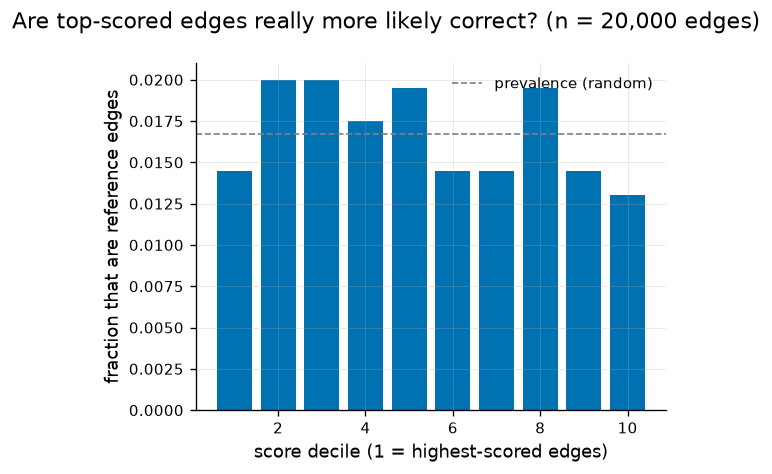
\includegraphics[width=0.85\linewidth]{../viz/calibration_cxg__10x-3-v2__homo-sapiens__entorhinal-cortex__06b91002.png}
\caption{-   (n = 20000 edges) - built from  motif\_prior.tsv.gz}
\end{figure}
\begin{figure}[H]\centering
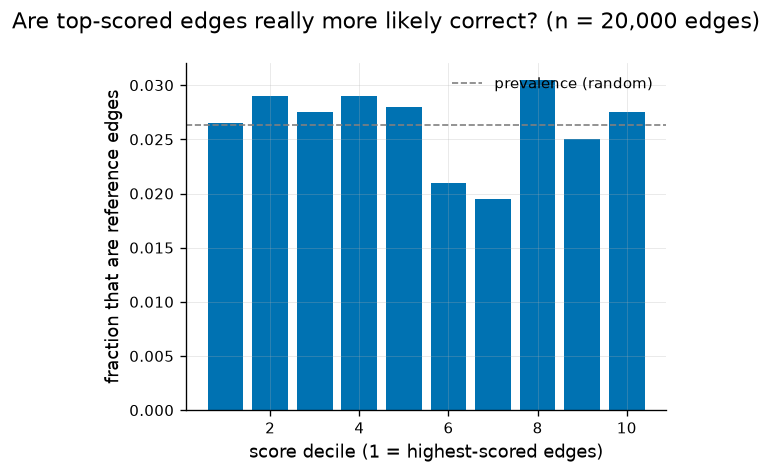
\includegraphics[width=0.85\linewidth]{../viz/calibration_cxg__10x-3-v2__homo-sapiens__peripheral-zone-of-prostate__df287f8d.png}
\caption{-   (n = 20000 edges) - built from  motif\_prior.tsv.gz}
\end{figure}
\begin{figure}[H]\centering
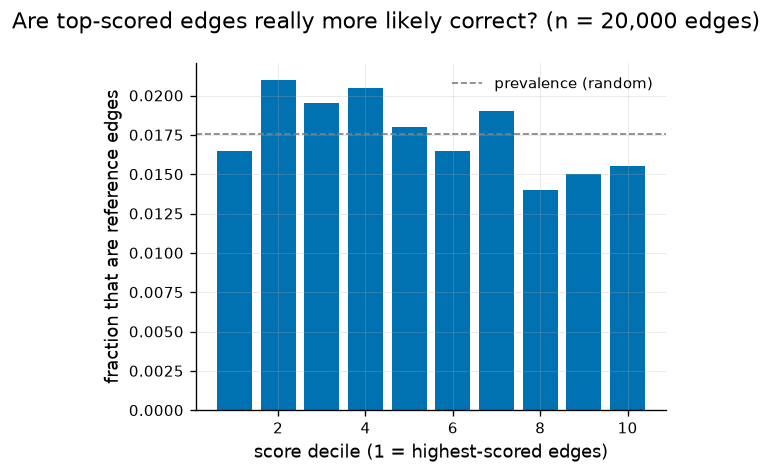
\includegraphics[width=0.85\linewidth]{../viz/calibration_cxg__10x-3-v2__homo-sapiens__superior-frontal-gyrus__b94e3bdf.png}
\caption{-   (n = 20000 edges) - built from  motif\_prior.tsv.gz}
\end{figure}
\begin{figure}[H]\centering
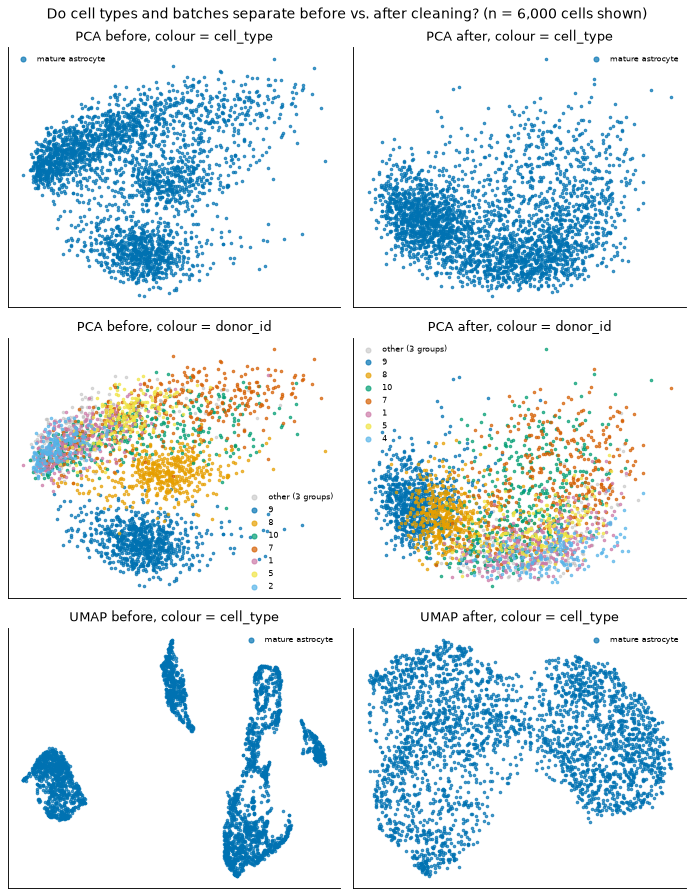
\includegraphics[width=0.85\linewidth]{../viz/embed_cxg__10x-3-v2__homo-sapiens__entorhinal-cortex__06b91002.png}
\caption{-   (n = 5500 cells) - built from  tasks.json (raw data)}
\end{figure}
\begin{figure}[H]\centering
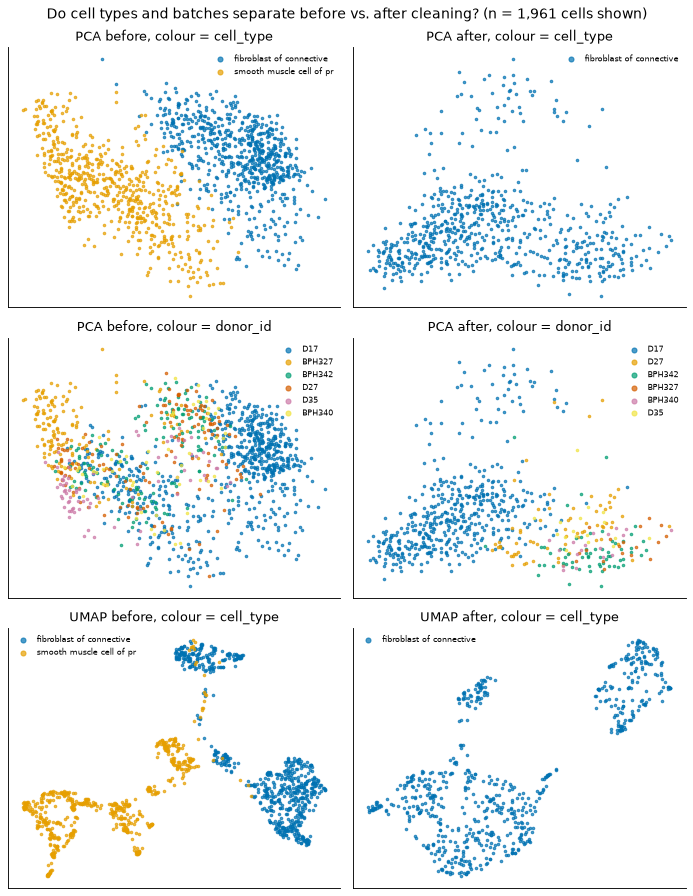
\includegraphics[width=0.85\linewidth]{../viz/embed_cxg__10x-3-v2__homo-sapiens__peripheral-zone-of-prostate__df287f8d.png}
\caption{-   (n = 1295 cells) - built from  tasks.json (raw data)}
\end{figure}
\begin{figure}[H]\centering
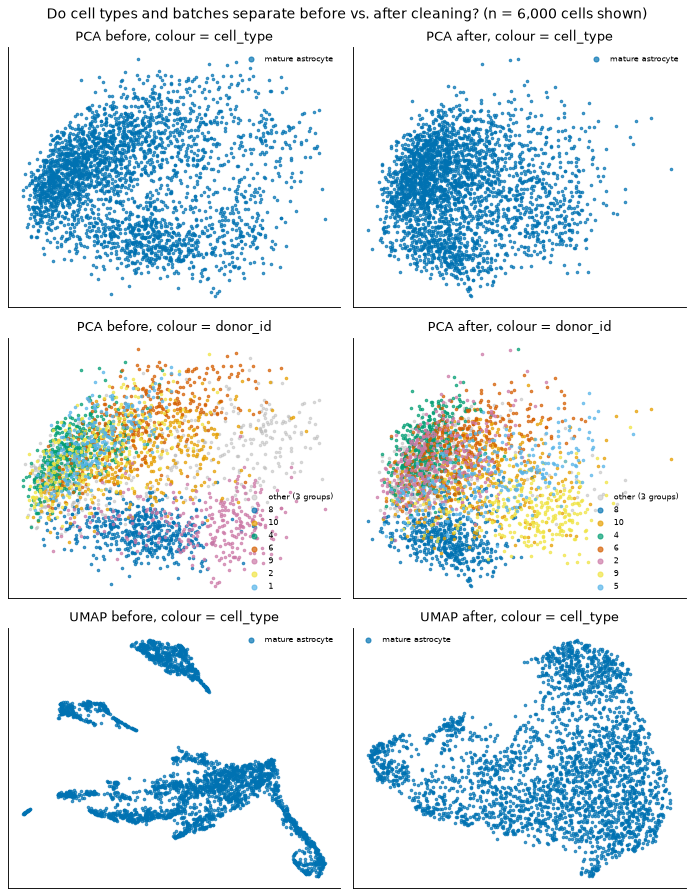
\includegraphics[width=0.85\linewidth]{../viz/embed_cxg__10x-3-v2__homo-sapiens__superior-frontal-gyrus__b94e3bdf.png}
\caption{-   (n = 5970 cells) - built from  tasks.json (raw data)}
\end{figure}
\begin{figure}[H]\centering
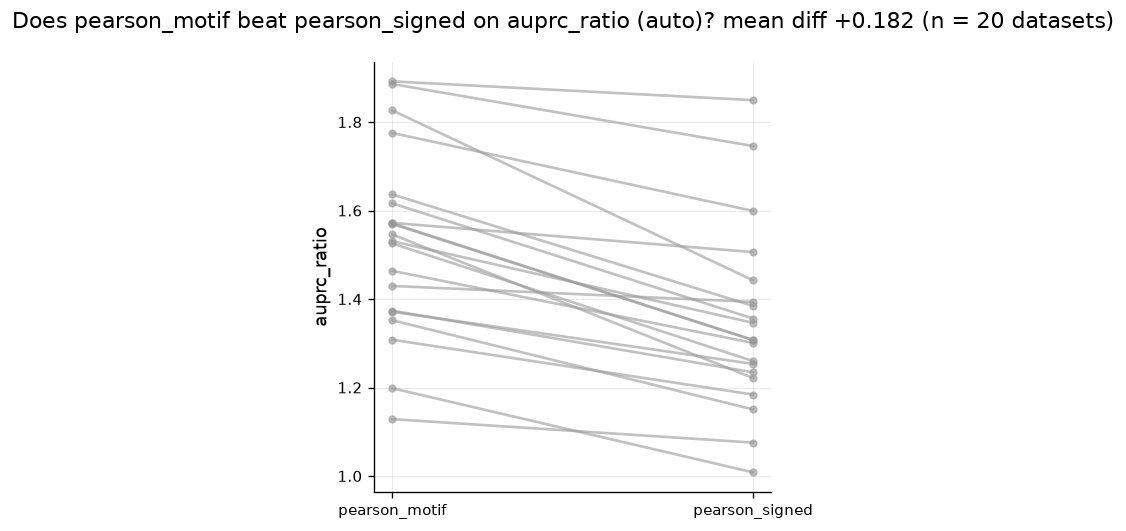
\includegraphics[width=0.85\linewidth]{../viz/lift_pearson_motif_vs_pearson_signed.png}
\caption{-   (n = 20 datasets) - built from  rows/ .json (pearson\_motif vs pearson\_signed)}
\end{figure}
\begin{figure}[H]\centering
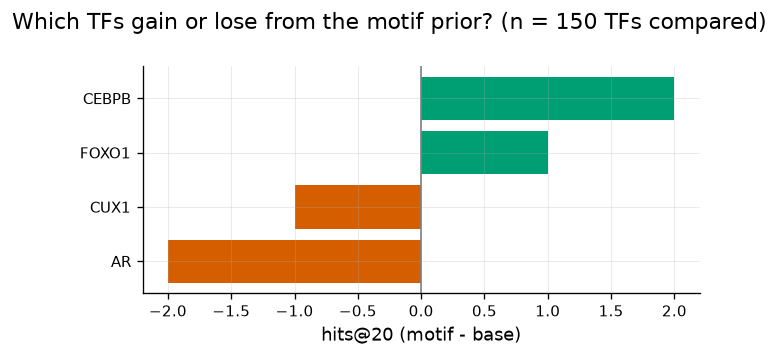
\includegraphics[width=0.85\linewidth]{../viz/motif_lift_cxg__10x-3-v2__homo-sapiens__entorhinal-cortex__06b91002_pearson_signed.png}
\caption{-   (n = shared TFs) - built from  pearson\_signed.tsv.gz vs pearson\_motif.tsv.gz}
\end{figure}
\begin{figure}[H]\centering
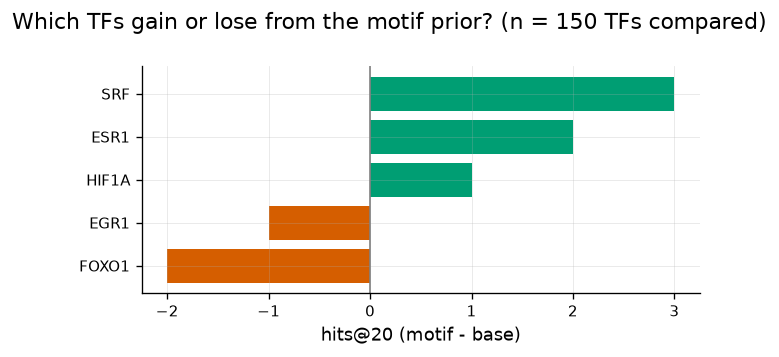
\includegraphics[width=0.85\linewidth]{../viz/motif_lift_cxg__10x-3-v2__homo-sapiens__peripheral-zone-of-prostate__df287f8d_pearson_signed.png}
\caption{-   (n = shared TFs) - built from  pearson\_signed.tsv.gz vs pearson\_motif.tsv.gz}
\end{figure}
\begin{figure}[H]\centering
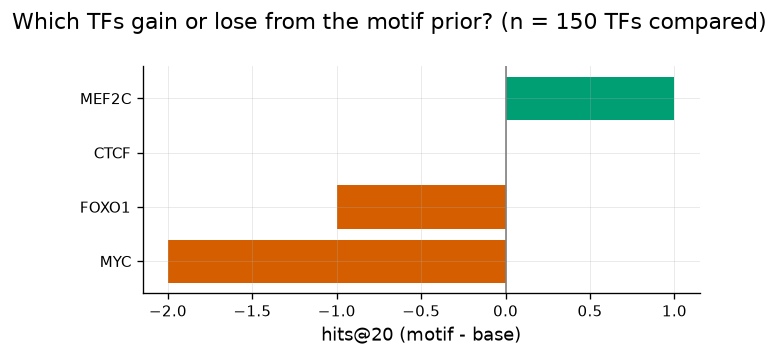
\includegraphics[width=0.85\linewidth]{../viz/motif_lift_cxg__10x-3-v2__homo-sapiens__superior-frontal-gyrus__b94e3bdf_pearson_signed.png}
\caption{-   (n = shared TFs) - built from  pearson\_signed.tsv.gz vs pearson\_motif.tsv.gz}
\end{figure}
\begin{figure}[H]\centering
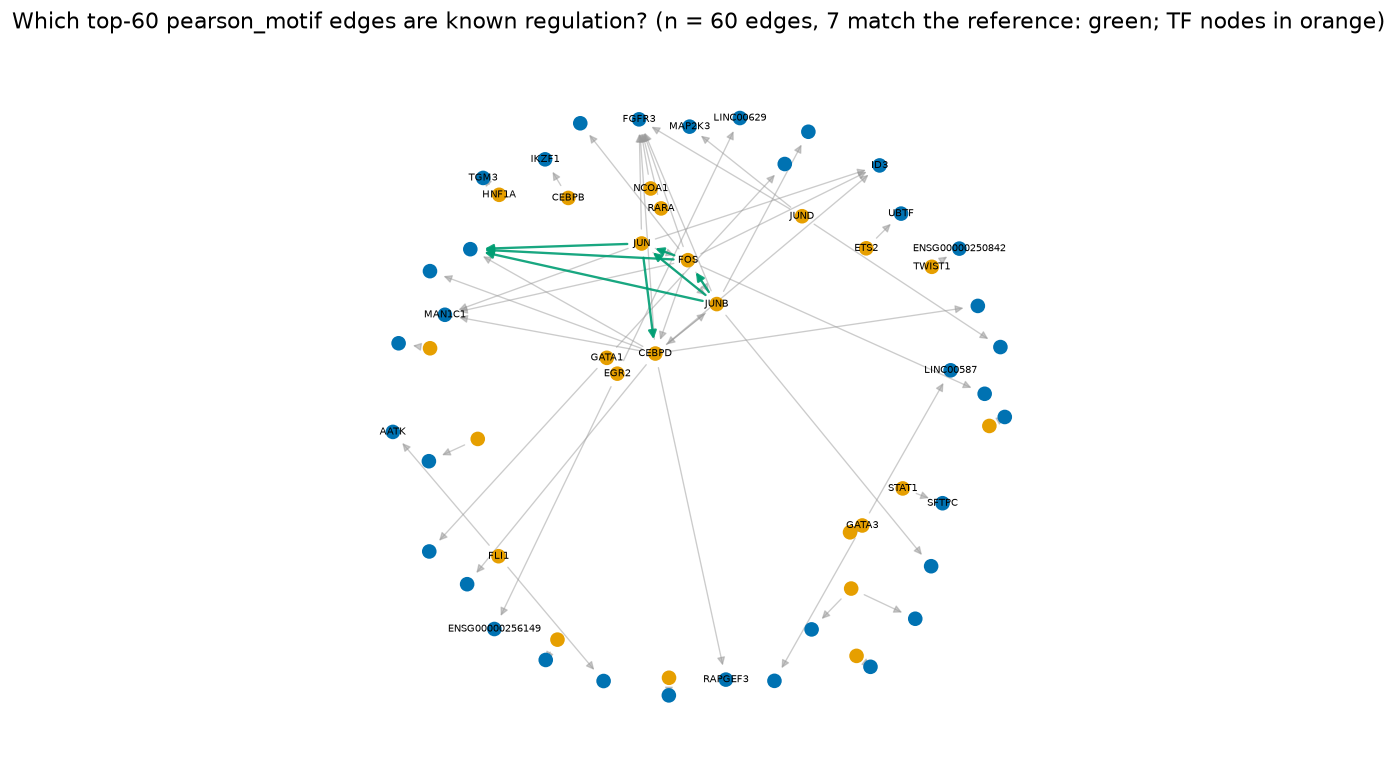
\includegraphics[width=0.85\linewidth]{../viz/network_cxg__10x-3-v2__homo-sapiens__entorhinal-cortex__06b91002.png}
\caption{-   (n = 60 edges) - built from  pearson\_motif.tsv.gz}
\end{figure}
\begin{figure}[H]\centering
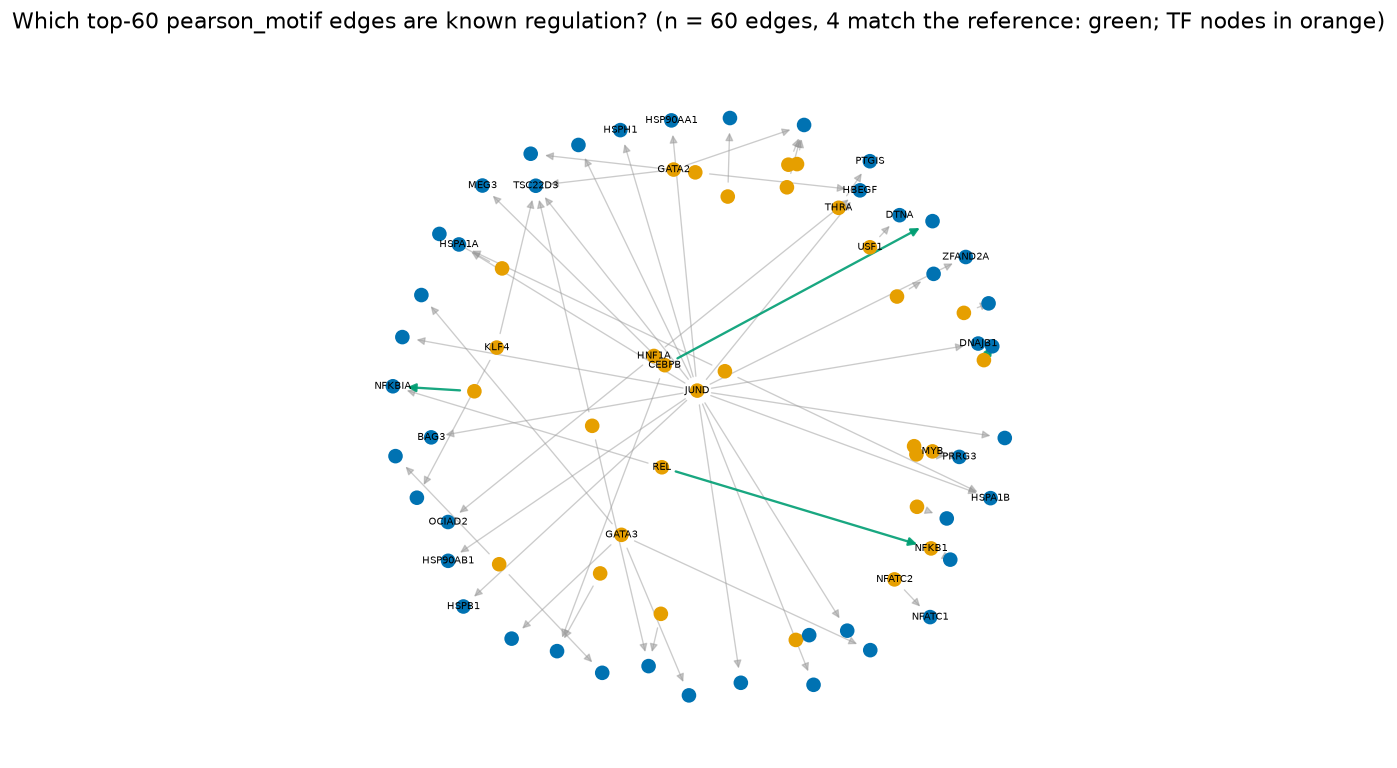
\includegraphics[width=0.85\linewidth]{../viz/network_cxg__10x-3-v2__homo-sapiens__peripheral-zone-of-prostate__df287f8d.png}
\caption{-   (n = 60 edges) - built from  pearson\_motif.tsv.gz}
\end{figure}
\begin{figure}[H]\centering
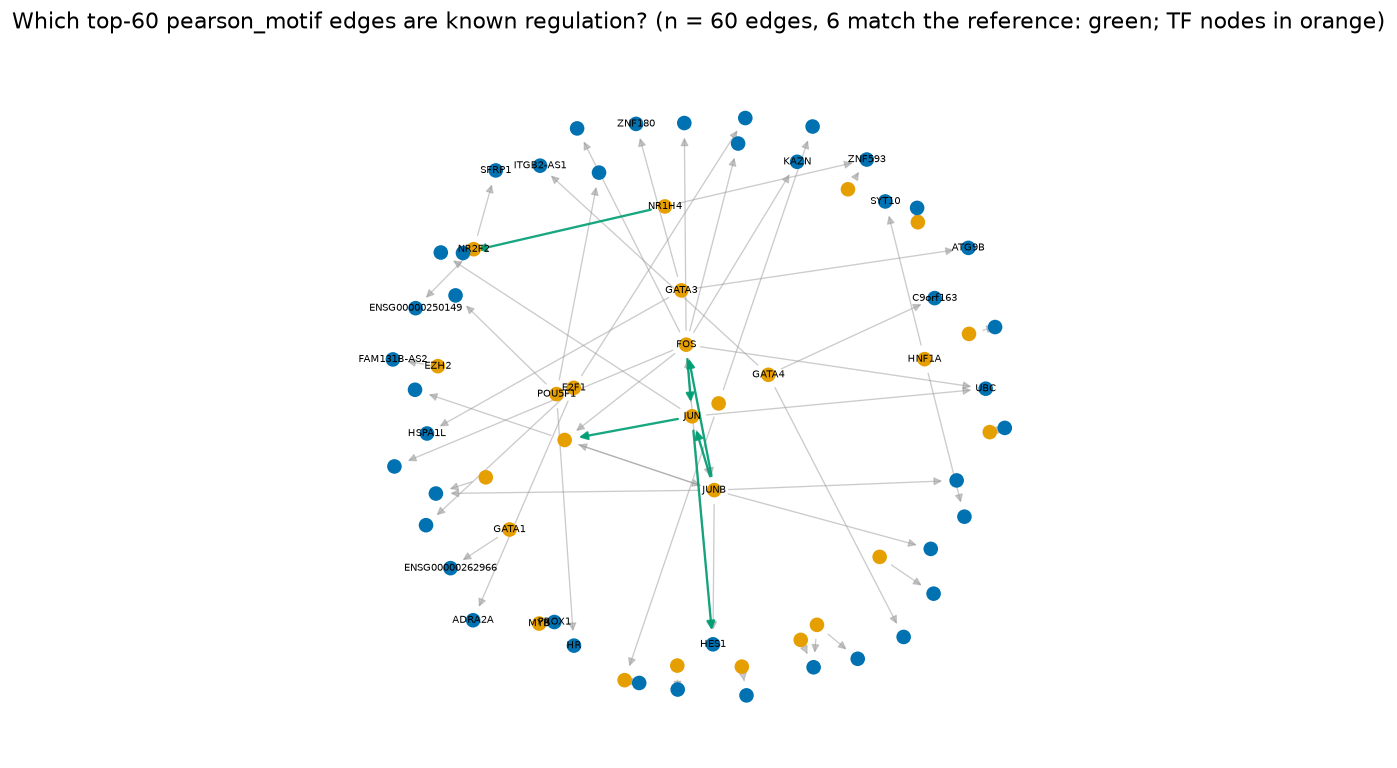
\includegraphics[width=0.85\linewidth]{../viz/network_cxg__10x-3-v2__homo-sapiens__superior-frontal-gyrus__b94e3bdf.png}
\caption{-   (n = 60 edges) - built from  pearson\_motif.tsv.gz}
\end{figure}
\begin{figure}[H]\centering
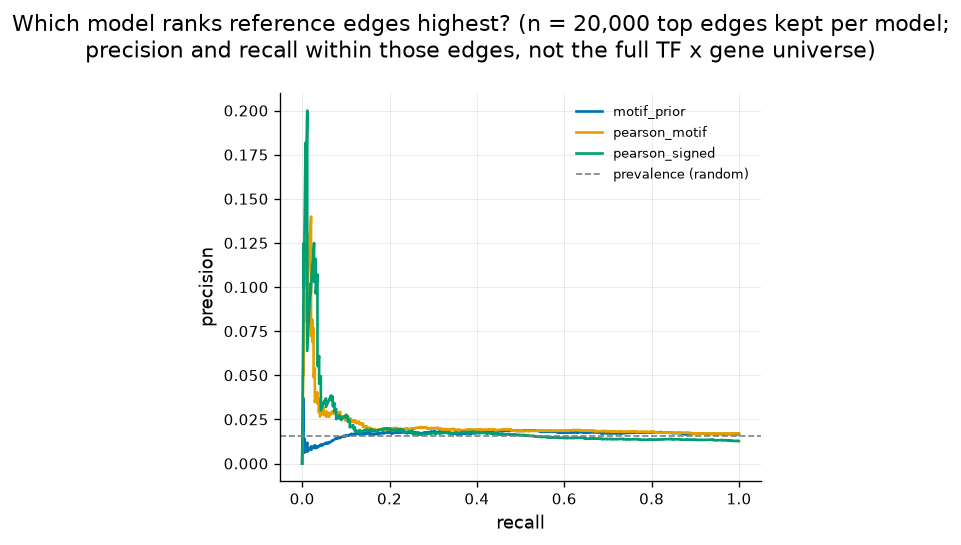
\includegraphics[width=0.85\linewidth]{../viz/pr_cxg__10x-3-v2__homo-sapiens__entorhinal-cortex__06b91002.png}
\caption{-   (n = 20000 edges) - built from  artifacts/cxg\_\_10x-3-v2\_\_homo-sapiens\_\_entorhinal-cortex\_\_06b91002/auto/ctx0}
\end{figure}
\begin{figure}[H]\centering
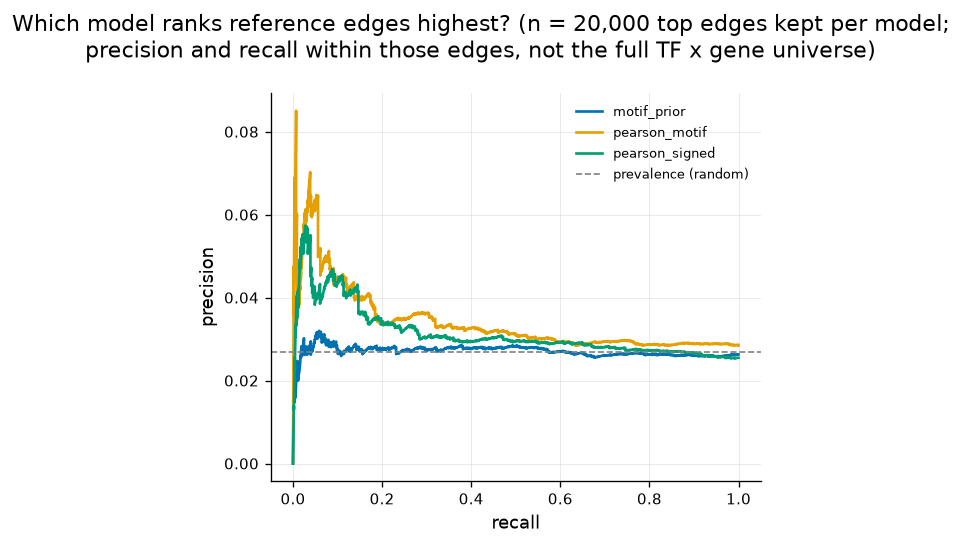
\includegraphics[width=0.85\linewidth]{../viz/pr_cxg__10x-3-v2__homo-sapiens__peripheral-zone-of-prostate__df287f8d.png}
\caption{-   (n = 20000 edges) - built from  artifacts/cxg\_\_10x-3-v2\_\_homo-sapiens\_\_peripheral-zone-of-prostate\_\_df287f8d/auto/ctx0}
\end{figure}
\begin{figure}[H]\centering
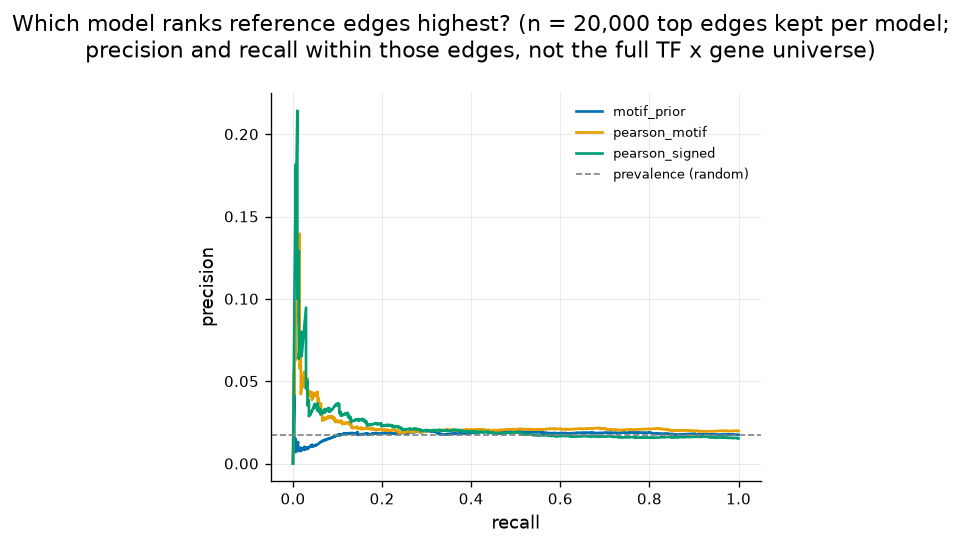
\includegraphics[width=0.85\linewidth]{../viz/pr_cxg__10x-3-v2__homo-sapiens__superior-frontal-gyrus__b94e3bdf.png}
\caption{-   (n = 20000 edges) - built from  artifacts/cxg\_\_10x-3-v2\_\_homo-sapiens\_\_superior-frontal-gyrus\_\_b94e3bdf/auto/ctx0}
\end{figure}
\begin{figure}[H]\centering
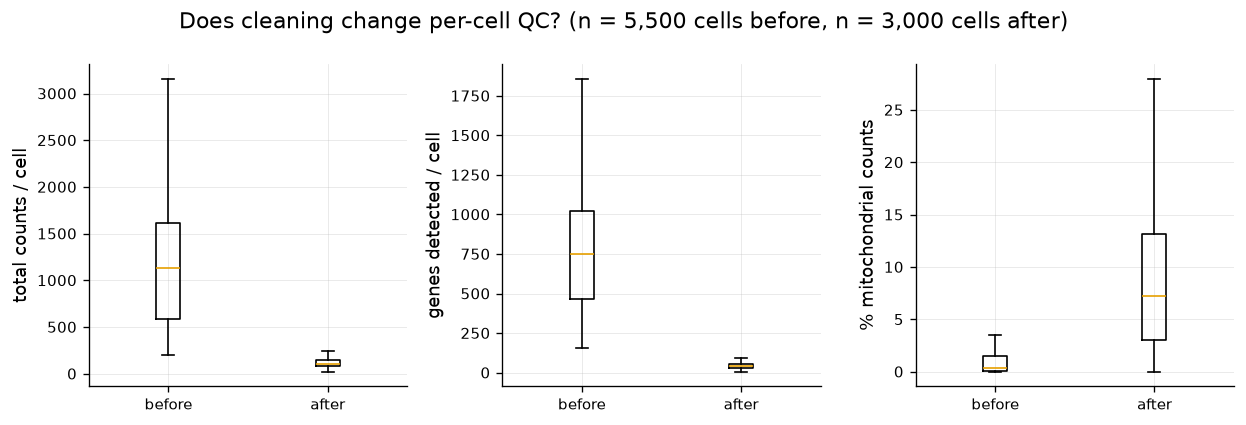
\includegraphics[width=0.85\linewidth]{../viz/qc_cxg__10x-3-v2__homo-sapiens__entorhinal-cortex__06b91002.png}
\caption{-   (n = 5500 cells) - built from  tasks.json (raw data)}
\end{figure}
\begin{figure}[H]\centering
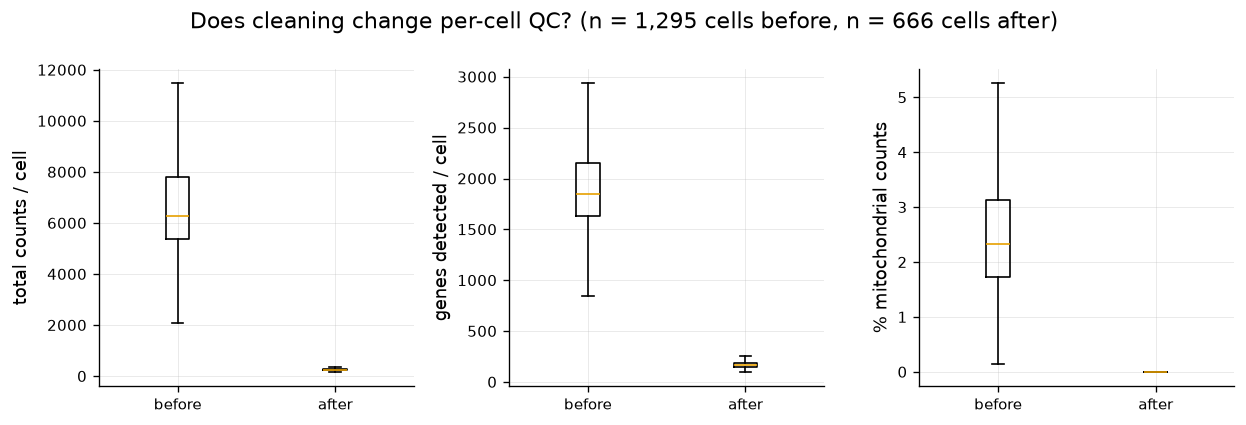
\includegraphics[width=0.85\linewidth]{../viz/qc_cxg__10x-3-v2__homo-sapiens__peripheral-zone-of-prostate__df287f8d.png}
\caption{-   (n = 1295 cells) - built from  tasks.json (raw data)}
\end{figure}
\begin{figure}[H]\centering
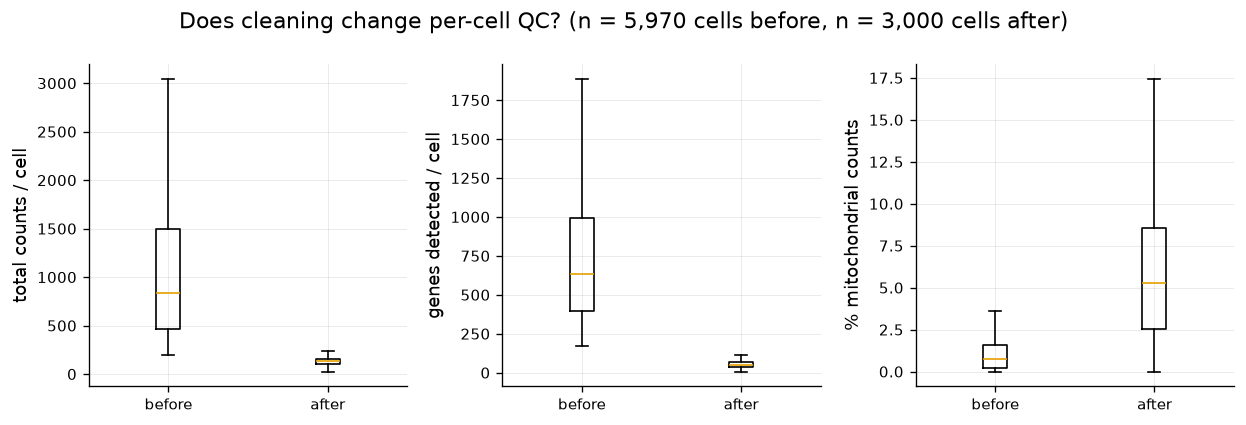
\includegraphics[width=0.85\linewidth]{../viz/qc_cxg__10x-3-v2__homo-sapiens__superior-frontal-gyrus__b94e3bdf.png}
\caption{-   (n = 5970 cells) - built from  tasks.json (raw data)}
\end{figure}
\begin{figure}[H]\centering
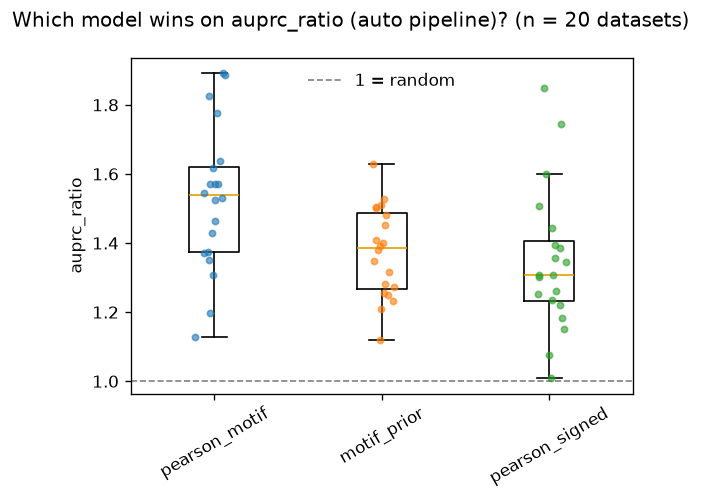
\includegraphics[width=0.85\linewidth]{../viz/scores_auprc_ratio_auto.png}
\caption{-   (n = 20 datasets) - built from  rows/ .json (auto/auprc\_ratio)}
\end{figure}
\begin{figure}[H]\centering
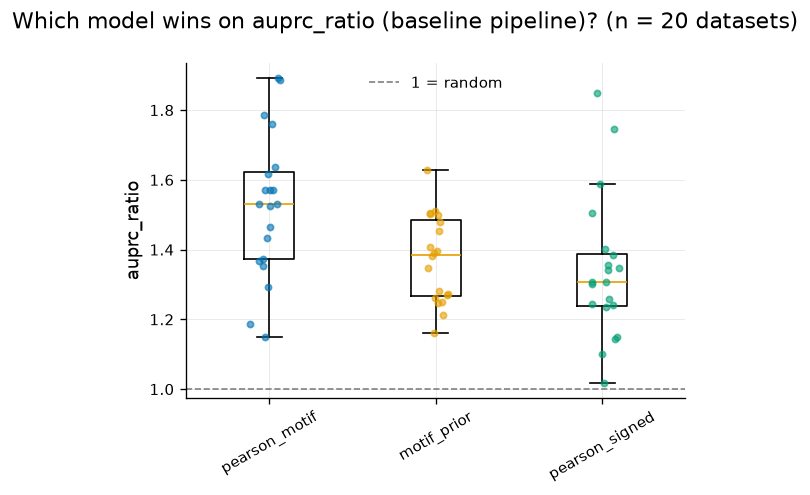
\includegraphics[width=0.85\linewidth]{../viz/scores_auprc_ratio_baseline.png}
\caption{-   (n = 20 datasets) - built from  rows/ .json (baseline/auprc\_ratio)}
\end{figure}
\begin{figure}[H]\centering
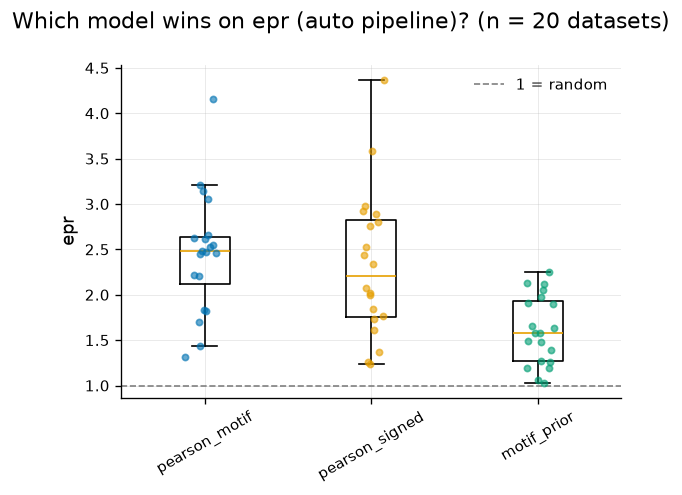
\includegraphics[width=0.85\linewidth]{../viz/scores_epr_auto.png}
\caption{-   (n = 20 datasets) - built from  rows/ .json (auto/epr)}
\end{figure}
\begin{figure}[H]\centering
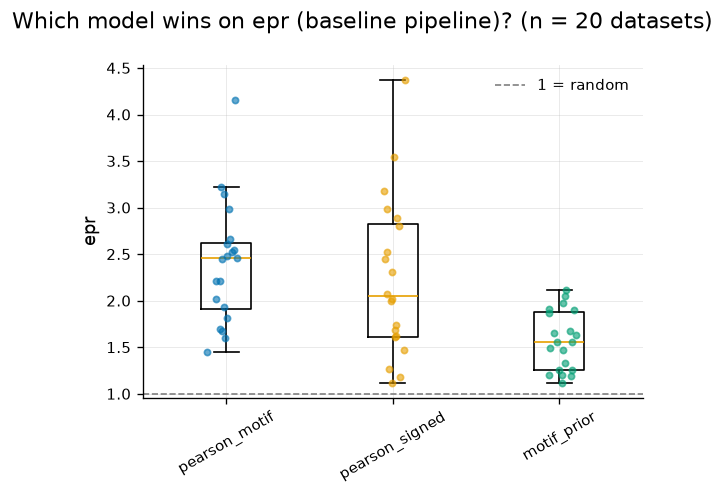
\includegraphics[width=0.85\linewidth]{../viz/scores_epr_baseline.png}
\caption{-   (n = 20 datasets) - built from  rows/ .json (baseline/epr)}
\end{figure}
\begin{figure}[H]\centering
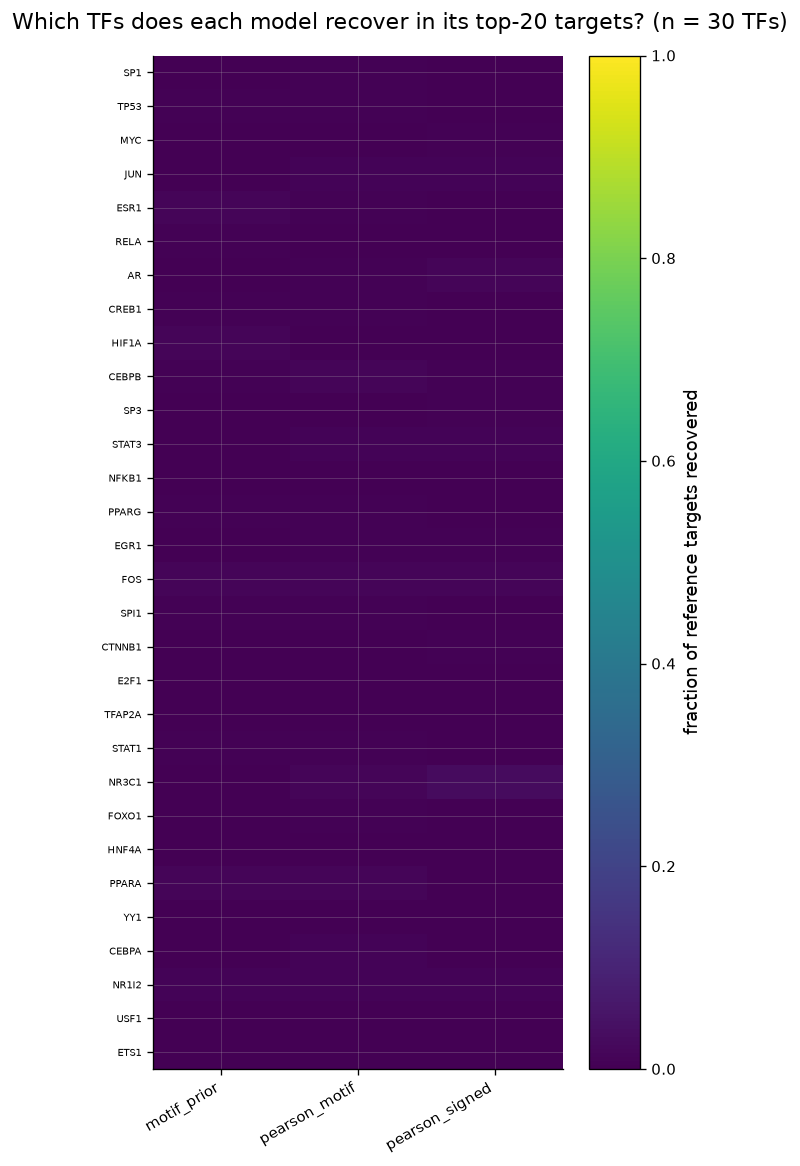
\includegraphics[width=0.85\linewidth]{../viz/tf_recovery_cxg__10x-3-v2__homo-sapiens__entorhinal-cortex__06b91002.png}
\caption{-   (n = up to 30 TFs) - built from  artifacts/cxg\_\_10x-3-v2\_\_homo-sapiens\_\_entorhinal-cortex\_\_06b91002/auto}
\end{figure}
\begin{figure}[H]\centering
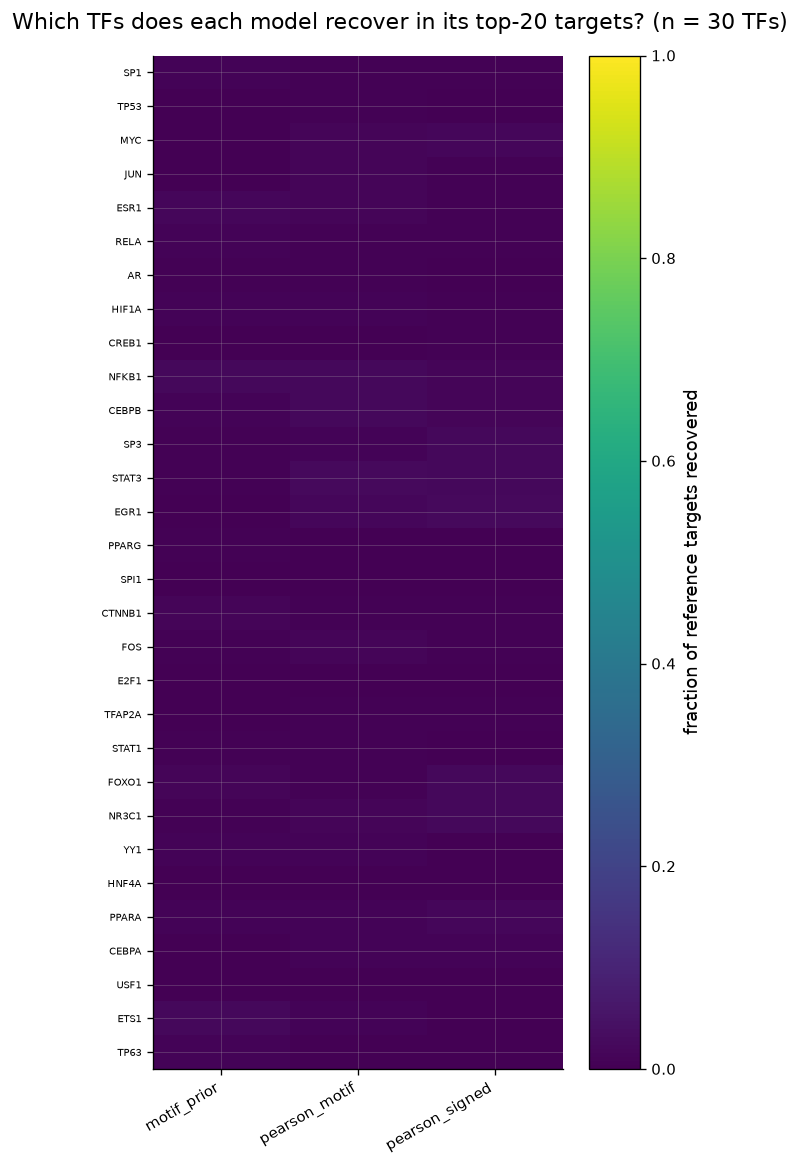
\includegraphics[width=0.85\linewidth]{../viz/tf_recovery_cxg__10x-3-v2__homo-sapiens__peripheral-zone-of-prostate__df287f8d.png}
\caption{-   (n = up to 30 TFs) - built from  artifacts/cxg\_\_10x-3-v2\_\_homo-sapiens\_\_peripheral-zone-of-prostate\_\_df287f8d/auto}
\end{figure}
\begin{figure}[H]\centering
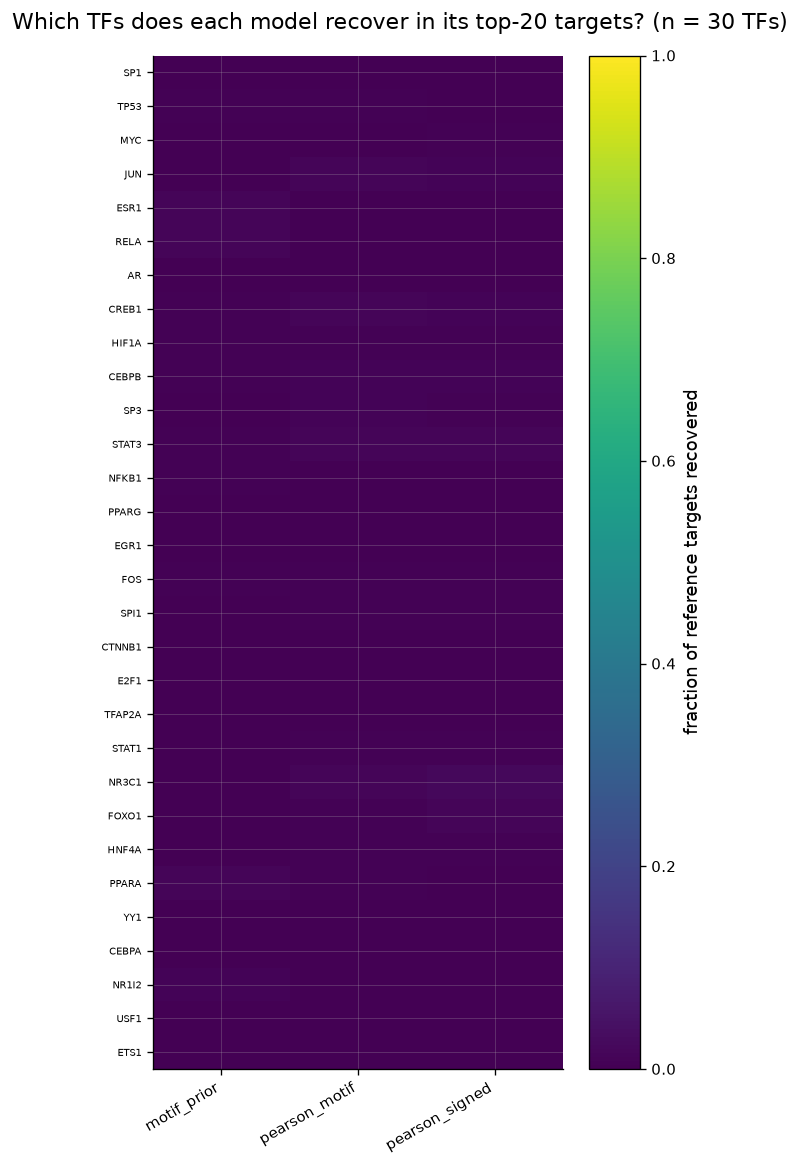
\includegraphics[width=0.85\linewidth]{../viz/tf_recovery_cxg__10x-3-v2__homo-sapiens__superior-frontal-gyrus__b94e3bdf.png}
\caption{-   (n = up to 30 TFs) - built from  artifacts/cxg\_\_10x-3-v2\_\_homo-sapiens\_\_superior-frontal-gyrus\_\_b94e3bdf/auto}
\end{figure}

\section{Limitations}
\begin{itemize}
\item Doublet calling fell back to the heuristic in 4 of 20 datasets.
\end{itemize}

\end{document}
